% !TEX root = ../../../main.tex
% 来源：中学数学实验教材·第三册（高中数学）
% 章节：任意角的三角函数 / 弧和角的概念及其度量
% 原始文件：6.tex，行 633-663
% 类型：tikz
% ---
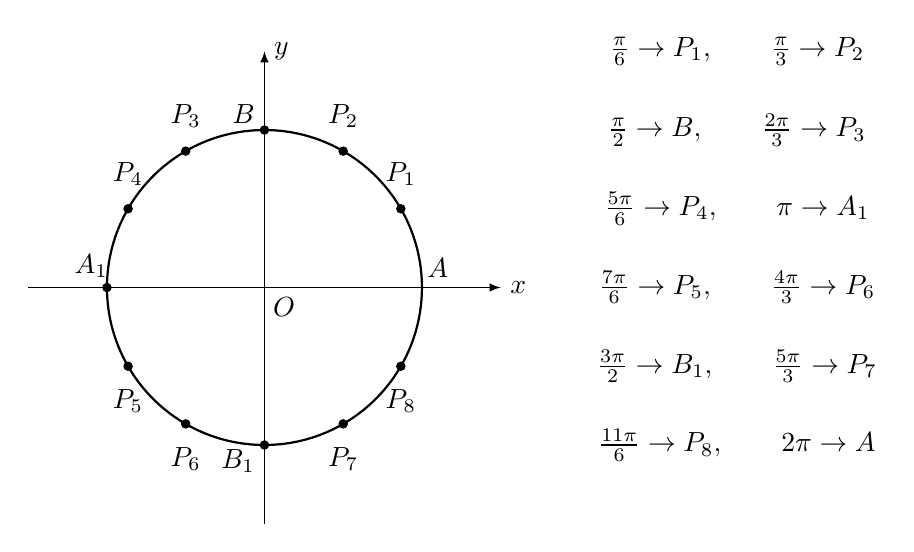
\begin{tikzpicture}[>=latex]
    \draw[->] (-3,0)--(3,0)node[right]{$x$};
    \draw[->] (0,-3)--(0,3)node[right]{$y$};
\draw[thick] (0,0) circle(2);

    \draw (1*30:2) [fill=black] circle (1.5pt) node[above=5pt]{$P_1$};
    \draw (2*30:2) [fill=black] circle (1.5pt) node[above=5pt]{$P_2$};
    \draw (3*30:2) [fill=black] circle (1.5pt);
    \draw (4*30:2) [fill=black] circle (1.5pt) node[above=5pt]{$P_3$};
    \draw (5*30:2) [fill=black] circle (1.5pt) node[above=5pt]{$P_4$};
    \draw (6*30:2) [fill=black] circle (1.5pt);
    \draw (7*30:2) [fill=black] circle (1.5pt) node[below=5pt]{$P_5$};
    \draw (8*30:2) [fill=black] circle (1.5pt) node[below=5pt]{$P_6$};
    \draw (9*30:2) [fill=black] circle (1.5pt);
    \draw (10*30:2) [fill=black] circle (1.5pt) node[below=5pt]{$P_7$};
    \draw (11*30:2) [fill=black] circle (1.5pt) node[below=5pt]{$P_8$};
   
\node at (2.2,0)[above]{$A$};   
\node at (-2.2,0)[above]{$A_1$};
\node at (0,2.2)[left]{$B$};   
\node at (0,-2.2)[left]{$B_1$};
\node at (0.25,-.25){$O$};  

\node at (6,3){$\frac{\pi}{6}\to P_1,\qquad \frac{\pi}{3}\to P_2$};
\node at (6,2){$ \frac{\pi}{2}\to B,\qquad \frac{2\pi}{3}\to P_3$};
\node at (6,1){$\frac{5\pi}{6}\to P_4,\qquad \pi\to A_1$};
\node at (6,0){$\frac{7\pi}{6}\to P_5,\qquad \frac{4\pi}{3}\to P_6$};
\node at (6,-1){$\frac{3\pi}{2}\to B_1,\qquad \frac{5\pi}{3}\to P_7$};
\node at (6,-2){$\frac{11\pi}{6}\to P_8,\qquad 2\pi\to A$};

\end{tikzpicture}
